\documentclass[12pt]{article}

% LuaLaTeX: fontspec + polyglossia для корректной работы с кириллицей
\usepackage{fontspec}
\usepackage{polyglossia}

\setmainlanguage{russian}

% Установка шрифтов с поддержкой кириллицы
\setmainfont{Times New Roman}

\usepackage[style=numeric, backend=biber]{biblatex} % Обязательный пакет для корректной сборки
\addbibresource{references.bib}
\usepackage{graphicx}        						% Графика
\usepackage[protrusion=false]{microtype}       		% Микротипографика
\usepackage{amssymb}        						% Математические символы
\usepackage{amsmath}        						% Математика
\usepackage{longtable}       						% Таблицы с разрывом страниц
\usepackage{tikz}           						% Рисование
\usepackage{circuitikz}     						% Электрические схемы
\usepackage{fix-cm}         						% Чтобы работал большой размер шрифта
\usepackage{anyfontsize}    						% Для любого размера шрифта
\usepackage{listings}       						% Для отображения кода
\usepackage{xcolor}         						% Для работы с цветами
\usepackage{subcaption}     						% Для подфигур
\usepackage{tabularx}       						% Для таблиц во всю ширину
\usepackage{array}          						% Для форматирования ячеек таблиц
\usepackage{pgfplots}       						% Для построения графиков
\pgfplotsset{compat=1.18}   						% Совместимость pgfplots
\usepackage{float}          						% Для точного позиционирования фигур

\usepackage{fancyhdr}                        % Колонтитулы
\usepackage[a4paper,left=30mm,right=15mm,top=20mm,bottom=20mm]{geometry}

% Оформление: поля, кегль 12pt задан, межстрочный 1.5, отступ 1,25 см,
% выравнивание по ширине, цвет — чёрный
\usepackage{setspace}                        % Для управления межстрочным интервалом
\usepackage{indentfirst}                     % Сделать отступ у первого абзаца после заголовка
\usepackage{ragged2e}                        % Команда \justifying для выравнивания по ширине

\setlength{\parindent}{1.25cm}              % Отступ в начале абзаца — 1,25 см
\onehalfspacing                              % Межстрочный интервал 1,5
\AtBeginDocument{\color{black}\justifying} % Чёрный шрифт и выравнивание по ширине

\title{
	Министерство науки и высшего образования Российской Федерации
	Федеральное государственное автономное образовательное учреждение 
	высшего образования

	«Национальный исследовательский университет
	«Московский институт электронной техники»

	Институт микроприборов и систем управления
	\vspace{2em}
}
\author{}
\date{}

\begin{document}

\maketitle
\thispagestyle{fancy}


\begin{raggedleft}
Отчёт по лабораторной работе №1
\end{raggedleft}
\begin{center}
\Large Однократные измерения	
\end{center}

\vspace{6em}

\begin{flushright}
	Выполнили студенты группы ЭН-25\\
	Андреев И. А.\\
	Анисимов А. С.\\
	Проверил преподаватель\\
	Туринцев К. А.
\end{flushright}

\fancyhf{}
\cfoot{Москва, 2026 г.}

\pagebreak

\section*{Содержание}

\begin{enumerate}
	\item TODO
\end{enumerate}

\pagebreak

\begin{center}
	\Large{\textbf{Лабораторная работа №1}}
\end{center}

\begin{center}
	\LARGE{\textbf{Однократные измерения}}
\end{center}

\large{\textbf{\textit{Цель работы}:} постановка измерительных экспериментов по оценке электрических параметров 
цепей при статических однократных измерениях с использованием цифрового мультиметра 
и источника питания с последующей оценкой погрешностей данных измерений.

\textbf{\textit{Необходимое оборудование}:} источник питания (Rigol DP811A), цифровой мультиметр (Rigol DM3058), макетная плата, 
кабели, перемычки, щупы.}

\section*{Теоритические данные}

\textbf{Однократные измерения} представляют собой доступный способ
оценки измеряемой величины, когда многократное повторение эксперимента 
нецелесообразно или ограничено техническими, временны́ ми
или ресурсными возможностями.

\textbf{Цифровые мультиметры} (рис. \ref{fig:multimeter}) – это многофункциональные измерительные 
приборы, предназначенные для измерения электрических параметров цепи по 
постоянному и переменному току.

Через входные разъемы \textbf{Input HI/LO} мультиметр подключается к
исследуемой цепи для измерений напряжения постоянного и переменного тока, 
электрического сопротивления и емкости, целостности цепи
и диодного теста. Для измерения силы постоянного и переменного тока
в большинстве мультиметров предусмотрен встроенный шунт, который
включается в исследуемую цепь с помощью разъема \textbf{Input I}. Разъемы
\textbf{Sense HI/LO} используются для высокоточного измерения электрического 
сопротивления исследуемой цепи по \textbf{4-проводной схеме} и для подключения 
внешних датчиков, например датчиков температуры.

\begin{figure}
\centering
\includegraphics[width=\textwidth]{multimeter1.png}
\caption{Цифровой мультиметр}
\label{fig:multimeter}
\end{figure}

Измерение мультиметром состоит из нескольких этапов, называемых 
измерительным циклом:

\begin{enumerate}
	\item Настройка аналогового тракта для измерения в определенном режиме.
	\item Калибровка аналого-цифрового преобразователя (АЦП), во время которой считывается 
	напряжение встроенного калибровочного источника опорного напряжения и сравнивается 
	с задаваемым значением, после чего корректируется значение коэффициента усиления 
	постоянного тока аналогового тракта.
	\item Установка нуля для компенсации систематических погрешностей мультиметра, 
	для чего отключается входной сигнал, считывается значение АЦП и вычитается полученное значение из последующих измерений входного 
	сигнала.
	\item Настройка АЦП и режима обработки считываемых значений вычислительным 
	устройством, от которого будут зависеть разрешение и скорость измерения.
	\item Многократное снятие показаний, их обработка (например,
	усреднение), передача в контроллер ввода/вывода для последующего
	вывода на дисплей. Измерительный цикл может быть запущен однократно 
	или работать без остановки — это определяется настройками
	мультиметра, задаваемыми через органы управления.
\end{enumerate}

Мультиметр измеряет напряжение путем подключения ко входам
\textbf{Input HI/LO} посредством щупов двух точек исследуемой электрической
цепи, между которыми необходимо определить разность потенциалов.
Выделяют режим измерения напряжения постоянного тока и режим
измерения напряжения переменного тока.

\textit{Напряжение постоянного тока (DC voltage)}. Мультиметр в режиме измерения напряжения 
постоянного тока работает по принципу прямого преобразования аналогового сигнала в 
цифровой. Входной сигнал, представляющий собой отмасштабированное постоянное напряжение,
поступает на вход АЦП, где преобразуется в цифровой код, отображаемый на экране 
устройства после его обработки (например, усреднения) в решающем устройстве.

\begin{figure}
\centering
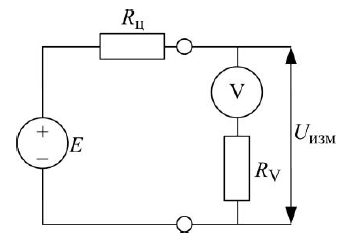
\includegraphics[width=\textwidth]{MethodAccuracy1.png}
\caption{Схема измерения напряжения мультиметром в режиме вольтметра}
\label{fig:methodaccuracy}
\end{figure}

При этом измеряемое мультиметром в режиме вольтметра напряжение (рис. 
\ref{fig:methodaccuracy}) можно записать в виде:

\begin{equation}
U_{\text{изм}} = U_{V} = E\frac{R_V}{R_V + R_{\text{ц}}}
\end{equation}

где $R_V$ — внутреннее сопротивление вольтметра, которое в идеальном и
недостижимом случае принимает значение бесконечности, а в современных 
средствах измерений — от 1 МОм и более. Именно из-за внутреннего 
сопротивления вольтметра, отличного по значению от бесконечности, 
возникает \textbf{методическая погрешность}, так как наша цепь превращается в 
делитель напряжения, а \textbf{методическая погрешность} может быть выражена как:

\begin{equation}
	\theta_m = U_V - E = E\left(\frac{R_V}{R_V + R_{\text{ц}}} - 1\right)
\end{equation}

\textit{Измерение силы постоянного тока (DC current)}. Для режимов работы мультиметра по измерению силы постоянного
и переменного тока предусмотрен разъем \textbf{Input I}. В режиме измерения силы постоянного 
тока мультиметр измеряет ток, протекающий через него, преобразуя его в напряжение 
с помощью шунтирующего резистора. Затем это напряжение подается на вход АЦП, 
и устройство отображает результат на экране.

\textit{Измерение электрического сопротивления}. Для измерения сопротивления мультиметр 
использует метод испытательного тока. В этом
режиме с источника образцового тока через измеряемый резистор пропускается 
испытательный ток и измеряется падение напряжения на исследуемой цепи. Далее, 
на основе полученного значения падения напряжения и априорно известного 
значения испытательного тока, решающее устройство мультиметра вычисляет искомое 
сопротивление цепи.

При измерении 2-проводным методом (рис. \ref{fig:2wireScheme}) на мультиметре возникает дополнительная погрешность 
из-за падения напряжения на проводах и контактах \textbf{Input HI/LO}:
$$
U_{\text{изм}} = I_{\text{исп}}(R_{\text{изм}} + 2R_{\text{пр}})
$$
При малых значениях сопротивления цепи (до 1 кОм) возникающая методическая погрешность 
может достигать нескольких процентов, поэтому для ее исключения используют 
4-проводную схему подключения цепи (рис. \ref{fig:4wireScheme}).

\begin{figure}
\centering
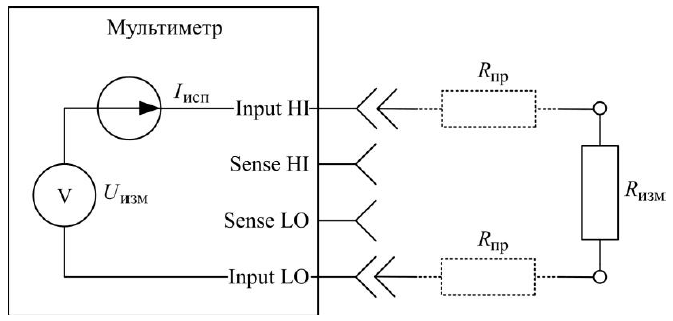
\includegraphics[width=\textwidth]{2wireScheme.png}
\caption{Схема 2-проводного измерения сопротивления}
\label{fig:2wireScheme}
\end{figure}

\begin{figure}
\centering
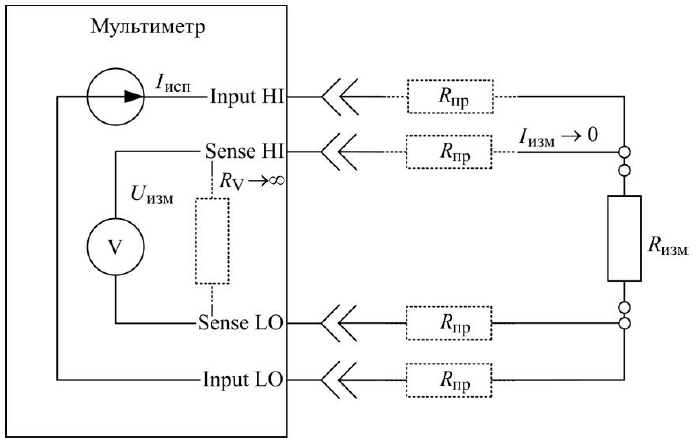
\includegraphics[width=\textwidth]{4wireScheme.png}
\caption{Схема 4-проводного измерения сопротивления}
\label{fig:4wireScheme}
\end{figure}

В данном режиме работы мультиметра испытательный постоянный
ток также подается по контактам \textbf{Input HI/LO}, а падение напряжения на
исследуемой цепи измеряется через контакты \textbf{Sense HI/LO}. Падение
напряжения на исследуемой цепи равно $U_R = I_{\text{исп}}R_{\text{изм}}$ и 
вызывает протекание небольшого измерительного тока через вольтметр:

\begin{equation}
I_{\text{изм}} = \frac{I_{\text{исп}} R_{\text{изм}}}{R_V + 2R_{\text{пр}}}
\end{equation}

Так как $U_{\text{изм}} = I_{\text{изм}} R_V$, то:

\begin{equation}
U_{\text{изм}} = \frac{I_{\text{исп}} R_V R_{\text{изм}}}{R_V + 2R_{\text{пр}}} = \frac{U_R R_V R_{\text{изм}}}{(R_V + 2R_{\text{пр}}) R_{\text{изм}}} = \frac{U_R R_V}{R_V + 2R_{\text{пр}}}
\end{equation}

При больших значениях внутреннего сопротивления вольтметра
(как правило, свыше 1 МОм) измеряемое значение падения напряжения
близко к падению напряжения на исследуемой цепи: $U_{\text{изм}} \approx U_R$. 
Следовательно, вычисляемое мультиметром сопротивление цепи не содержит
методической погрешности влияния сопротивления проводов и контактов.

\begin{center}
	\LARGE{\textbf{Ход работы}}
\end{center}

\section{Измерение температуры окружающего воздуха с помощью термистора}

\begin{figure}[H]
\centering

\includegraphics[width=\textwidth]{1experiment.png}
\caption{Схема измерения сопротивления термистора}
\label{fig:thermistor}
\end{figure}

\begin{center}
	\begin{tabularx}{\textwidth}{|>{\centering\arraybackslash}X|>{\centering\arraybackslash}X|}
		\hline
		Показания мультиметра в режиме измерения термистора типа TR2WR, $^\circ$C & 
		Показания мультиметра в режиме измерения TR при 2-проводной схеме, кОм \\
		\hline
		--- & 10,8370 \\
		\hline
	\end{tabularx}
\end{center}

\subsection{Расчёт погрешности измерения сопротивления}

Прибор Rigol DM3058 — прецизионный 5.5-разрядный мультиметр. 
Для диапазона \textbf{20 кОм} погрешность при $25^\circ\text{C} \pm 5^\circ\text{C}$ согласно 
спецификации составляет:
\begin{equation}
\Delta_{\text{приб}} = \pm(0,020\% \text{ от показания} + 0,003\% \text{ от диапазона})
\end{equation}

Абсолютная инструментальная погрешность прибора:
\begin{equation*}
\Delta_{\text{приб}} = \pm(10837 \cdot \frac{0,020}{100} + 20000 \cdot \frac{0,003}{100}) = \pm(2,1674 + 0,6) = \pm 2,7674 \text{ Ом}
\end{equation*}

В режиме 2WR мультиметр добавляет 
к результату сопротивление щупов $2R_{\text{пр}}$. Типичное значение сопротивления 
проводов и контактов составляет $0,1 \dots 0,3 \text{ Ом}$. Принимаем среднее значение $R_{\text{пр}} = 0,2 \text{ Ом}$.

\begin{equation*}
	\Delta_{\text{м}} = 2R_{\text{пр}} = 0,4 \text{ Ом}
\end{equation*}

Относительная погрешность измерения сопротивления термистора:

\begin{equation*}
\delta = \frac{\Delta_{\text{приб}} + \Delta_{\text{м}}}{R_{\text{изм}}} \cdot 100\% = \frac{2,7674 + 0,4}{10837,4} \cdot 100\% \approx 0,0292\%
\end{equation*}

Величина сопротивления термистора с учетом погрешности измерения:

\begin{equation*}
R_{\text{изм}} = R \pm (\Delta_{\text{приб}} + \Delta_{\text{м}}) = (10837,4 \pm 3,2) \text{ Ом}
\end{equation*}

\section{Измерение параметров цепи светодиода и резистора}

\subsection{Измерение входного напряжения цепи $U_{\text{вх}}$}

\begin{figure}[H]
\centering

\includegraphics[width=\textwidth]{2experiment.png}
\caption{Схема измерения входного напряжения цепи $U_{\text{вх}}$}
\label{fig:led1}
\end{figure}

\begin{center}
	\begin{tabularx}{\textwidth}{|>{\centering\arraybackslash}X|>{\centering\arraybackslash}X|>{\centering\arraybackslash}X|>{\centering\arraybackslash}X|>{\centering\arraybackslash}X|}
		\hline
		Диапазон измерений, В & 
		Скорость измерения, изм/с & 
		Входное сопротивление мультиметра, МОм & 
		Показания мультиметра, В & 
		Температура окружающего воздуха, $^\circ$С \\
		\hline
		20 & S & $10$ & 4,9770 & $\approx 25$ \\
		\hline
	\end{tabularx}
\end{center}

Для расчёта погрешности измерения постоянного напряжения воспользуемся паспортными 
данными прибора \textbf{Rigol DM3058}. Согласно спецификации DM3058 для диапазона $20 \text{ В}$ предел допускаемой основной 
погрешности составляет:

\begin{equation}
\Delta U_{\text{приб}} = \pm(0,015\% \text{ от показания} + 0,004\% \text{ от диапазона})
\end{equation}

Расчёт абсолютной приборной погрешности:

\begin{equation*}
\Delta U_{\text{приб}} = \pm(4,9770 \cdot \frac{0,015}{100} + 20 \cdot \frac{0,004}{100}) = \pm(0,00074655 + 0,0008) \approx \pm 1,5 \text{ мВ}
\end{equation*}

Расчёт относительной погрешности:

\begin{equation*}
\delta U = \frac{\Delta U_{\text{приб}}}{U_{\text{изм}}} \cdot 100\% = \frac{0,00155}{4,9770} \cdot 100\% \approx 0,031\%
\end{equation*}

Измеренное значение входного напряжения на макетной плате:
\begin{equation*}
U_{\text{вх}} = (4,9770 \pm 0,0015) \text{ В}
\end{equation*}

\subsection{Измерение силы тока $I_{\text{вх}}$}

\begin{figure}[H]
\centering
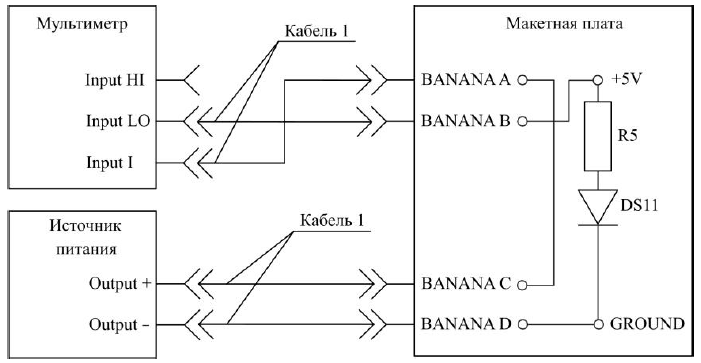
\includegraphics[width=\textwidth]{3experiment.png}
\caption{Схема измерения силы тока $I_{\text{вх}}$}
\label{fig:led2}
\end{figure}

\begin{center}
	\begin{tabularx}{\textwidth}{|>{\centering\arraybackslash}X|>{\centering\arraybackslash}X|>{\centering\arraybackslash}X|>{\centering\arraybackslash}X|>{\centering\arraybackslash}X|}
		\hline
		Диапазон измерений, мA & 
		Скорость измерения, изм/с & 
		Сопротивление внутреннего шунта, Ом & 
		Показания мультиметра, мA & 
		Температура окружающего воздуха, $^\circ$С \\
		\hline
		20 & S & $1$ & 9,0888 & $\approx 25$ \\
		\hline
	\end{tabularx}
\end{center}

Для расчёта погрешности измерения силы постоянного тока воспользуемся паспортными 
данными прибора Rigol DM3058. Согласно спецификации
DM3058 для диапазона 20 В предел допускаемой основной погрешности со
ставляет:

\begin{equation*}
\Delta I_{\text{приб}} = \pm (0,050\% \cdot I_{\text{изм}} + 0,005\% \cdot I_{\text{предела}})
\end{equation*}

Расчёт абсолютной приборной погрешности:

\begin{equation*}
\Delta I_{\text{приб}} = \pm(9,0888 \cdot \frac{0,050}{100} + 20 \cdot \frac{0,005}{100}) = \pm(0,0045444 + 0,001) \approx \pm 5,5 \text{ мкА}
\end{equation*}

Расчёт относительной погрешности:

\begin{equation*}
\delta I = \frac{\Delta I_{\text{приб}}}{I_{\text{изм}}} \cdot 100\% = \frac{0,00554}{9,0888} \cdot 100\% \approx 0,061\%
\end{equation*}

Измеренное значение силы тока в цепи светодиода:
\begin{equation*}
I_{\text{вх}} = (9,0888 \pm 0,0055) \text{ мА}
\end{equation*}

\subsection{Измерение падения напряжения на резисторе R5}

\begin{figure}[H]
\centering
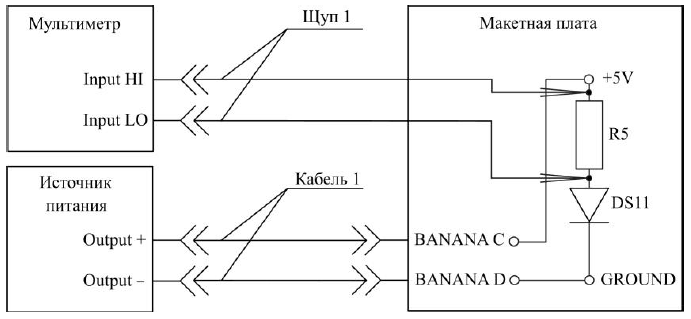
\includegraphics[width=\textwidth]{4experiment.png}
\caption{Схема измерения падения напряжения на резисторе R5}
\label{fig:resistor}
\end{figure}

\begin{center}
	\begin{tabularx}{\textwidth}{|>{\centering\arraybackslash}X|>{\centering\arraybackslash}X|>{\centering\arraybackslash}X|>{\centering\arraybackslash}X|>{\centering\arraybackslash}X|}
		\hline
		Диапазон измерений, В & 
		Скорость измерения, изм/с & 
		Входное сопротивление мультиметра, МОм & 
		Показания мультиметра, В & 
		Температура окружающего воздуха, $^\circ$С \\
		\hline
		20 & S & $10$ & 3,0650 & $\approx 25$ \\
		\hline
	\end{tabularx}
\end{center}

Расчёт абсолютной приборной погрешности:

\begin{equation*}
\Delta U_{\text{приб}} = \pm(3,0650 \cdot \frac{0,015}{100} + 20 \cdot \frac{0,004}{100}) = \pm(0,00045975 + 0,0008) \approx \pm 1,3 \text{ мВ}
\end{equation*}

Расчёт относительной погрешности:

\begin{equation*}
\delta U = \frac{\Delta U_{\text{приб}}}{U_{\text{изм}}} \cdot 100\% = \frac{0,00126}{3,0650} \cdot 100\% \approx 0,041\%
\end{equation*}

Измеренное значение падения напряжения на резисторе R5​:
\begin{equation*}
U_{R5} = (3,0650 \pm 0,0013) \text{ В}
\end{equation*}

\section{Измерение сопротивления резисторов}

\begin{figure}[H]
\centering
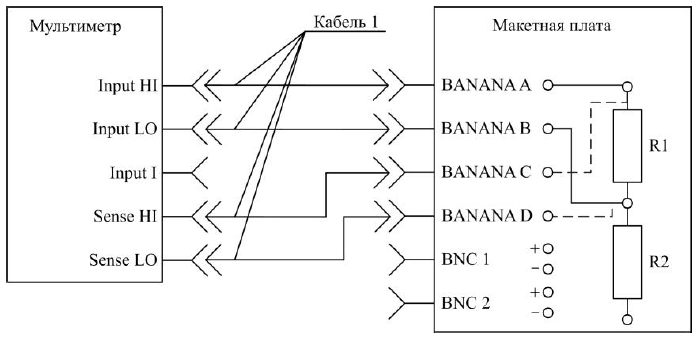
\includegraphics[width=\textwidth]{5experiment.png}
\caption{Схема измерения сопротивления на резисторе R1}
\label{fig:resistor2}
\end{figure}

\subsection{Измерение сопротивления резистора R1}

\begin{center}
	\begin{tabularx}{\textwidth}{|>{\centering\arraybackslash}X|>{\centering\arraybackslash}X|>{\centering\arraybackslash}X|>{\centering\arraybackslash}X|>{\centering\arraybackslash}X|>{\centering\arraybackslash}X|}
		\hline
		Диапазон измерений, кОм & 
		Скорость измерения, изм/с & 
		Сила испытательного тока, мА & 
		Показания мультиметра, кОм & 
		Показания мультиметра, Ом & 
		Температура окружающего воздуха,$^\circ$С \\
		\cline{4-5}
		& & & 2WR & 4WR & \\
		\hline
		20 & S & --- & 6,9218 & 6,9198 & $ \approx 25 $ \\
		\hline
	\end{tabularx}
\end{center}

Согласно паспортным данным DM3058 для диапазона 20 кОм:
\begin{equation*}
\Delta R_{\text{паспорт}} = \pm (0,020\% \cdot R_{\text{изм}} + 0,003\% \cdot R_{\text{предела}})
\end{equation*}

Для 4-проводной схемы (4WR), исключающей сопротивление щупов:

Расчёт абсолютной приборной погрешности:
\begin{equation*}
\Delta R_{1(4WR)} = \pm(6,9198 \cdot \frac{0,020}{100} + 20 \cdot \frac{0,003}{100}) = \pm(0,00138396 + 0,0006) \approx \pm 0,0020 \text{ кОм}
\end{equation*}

Расчёт относительной погрешности:
\begin{equation*}
\delta R_1 = \frac{\Delta R_{1(4WR)}}{R_{1(4WR)}} \cdot 100\% = \frac{0,00198}{6,9198} \cdot 100\% \approx 0,029\%
\end{equation*}

Измеренное значение сопротивления R1​:
\begin{equation*}
R_1 = (6,9198 \pm 0,0020) \text{ кОм}
\end{equation*}

Разница между двухпроводной (2WR) и четырехпроводной (4WR) схемами обусловлена 
сопротивлением соединительных проводов и контактов $R_{\text{пр}}$.

\begin{equation*}
R_{\text{п1}} = R_{1(2WR)} - R_{1(4WR)} = 6,9218 - 6,9198 = 0,0020 \text{ кОм} = 2,0 \text{ Ом}
\end{equation*}

\subsection{Измерение сопротивления резистора R2}

\begin{center}
	\begin{tabularx}{\textwidth}{|>{\centering\arraybackslash}X|>{\centering\arraybackslash}X|>{\centering\arraybackslash}X|>{\centering\arraybackslash}X|>{\centering\arraybackslash}X|>{\centering\arraybackslash}X|}
		\hline
		Диапазон измерений, кОм & 
		Скорость измерения, изм/с & 
		Сила испытательного тока, мА & 
		Показания мультиметра, кОм & 
		Показания мультиметра, кОм & 
		Температура окружающего воздуха,$^\circ$С \\
		\cline{4-5}
		& & & 2WR & 4WR & \\
		\hline
		20 & S & --- & 1,07132 & 0,99143 & $ \approx 25 $ \\
		\hline
	\end{tabularx}
\end{center}

Для 4-проводной схемы (4WR):

Расчёт абсолютной приборной погрешности:
\begin{equation*}
\Delta R_{2(4WR)} = \pm(0,99143 \cdot \frac{0,020}{100} + 20 \cdot \frac{0,003}{100}) = \pm(0,000198286 + 0,0006) \approx \pm 0,00080 \text{ кОм}
\end{equation*}

Расчёт относительной погрешности:
\begin{equation*}
\delta R_2 = \frac{\Delta R_{2(4WR)}}{R_{2(4WR)}} \cdot 100\% = \frac{0,000798}{0,99143} \cdot 100\% \approx 0,081\%
\end{equation*}

Измеренное значение сопротивления R2​:
\begin{equation*}
R_2 = (0,99143 \pm 0,00080) \text{ кОм}
\end{equation*}

Разница между двухпроводной (2WR) и четырехпроводной (4WR) схемами обусловлена 
сопротивлением соединительных проводов и контактов $R_{\text{пр}}$.

\begin{equation*}
R_{\text{п2}} = R_{2(2WR)} - R_{2(4WR)} = 1,07132 - 0,99143 = 0,07989 \text{ кОм} \approx 79,9 \text{ Ом}
\end{equation*}

\section{}

\end{document}